\documentclass[conference]{IEEEtran}
\IEEEoverridecommandlockouts
% The preceding line is only needed to identify funding in the first footnote. If that is unneeded, please comment it out.
\usepackage{cite}
\usepackage{amsmath,amssymb,amsfonts}
\usepackage{algorithmic}
\usepackage{graphicx}
\usepackage{caption}
\usepackage{textcomp}
\usepackage{xcolor}
\usepackage[utf8]{inputenc}
\usepackage{tabularx}
\def\BibTeX{{\rm B\kern-.05em{\sc i\kern-.025em b}\kern-.08em
    T\kern-.1667em\lower.7ex\hbox{E}\kern-.125emX}}
\begin{document}

\title{Development of Drones and Their Integration into Educational Robotics}

%%\author{Gustavo da Silva Nascimento Costa$^{1}$, João Vitor Nascimento$^{2}$, Jeovana Miranda Souza$^{3}$, Rafael Gomes de \\ Oliveira$^{4}$, Sávio Pessôa Afonso$^{5}$, Rian Cesar Oliveira Souza$^{6}$, Leandro Gonçalves dos Santos$^{7}$, \\and Fábio Santos Lima$^{8}$}

\maketitle

\begin{abstract}
The Educa Drones project at the Instituto Federal Baiano - Campus Guanambi employs STEAM technology within an interdisciplinary educational robotics context, focusing on rotary-wing drones such as the IF450 and Colibri versions, all based on open hardware. Students and teachers can explore complex concepts by building and operating these drones, which are modeled in Tinkercad, 3D-printed using PETG polymer, and feature a modular and robust design with advanced electronic components and telemetry via ESP32 radio. This initiative enhances learning, promotes entrepreneurship and innovation, and introduces a new business model in the academic and corporate landscape.
\end{abstract}

\begin{IEEEkeywords}
Remotely Piloted Aircraft, Educational Robotics, F450, Multirotor, Quadcopter, Modularity.
\end{IEEEkeywords}

\section{Introduction}

Brazil currently faces various challenges related to deficiencies in its public educational system. According to the results of the 2023 Program for International Student Assessment (PISA), more than 50\% of 15-year-old students lack basic proficiency in mathematics, science, and language \cite{b6}. This situation has been deteriorating since 2009.

In light of this, finding methods to encourage student learning has become essential. The use of technological resources for pedagogical purposes in educational institutions has gained increasing interest as a means to enhance the teaching and learning process \cite{b12}.

In the field of educational robotics, one such technological resource is the remotely piloted aircraft, commonly known as a drone. Drones provide opportunities to explore concepts in physics and mathematics, such as flight dynamics, force, thrust, Newton’s laws, distance, height, angles, and trigonometry, among others \cite{b11}. These are topics that are often difficult to grasp within the traditional teaching paradigm.

In addition, building these devices enables students to understand and apply basic and advanced concepts in electronics, chemistry, engineering, and programming \cite{b12}. These are fundamental skills for preparing professionals to compete in a globalized market. From this perspective, the Educa Drones project was established at the Instituto Federal de Educação, Ciência e Tecnologia Baiano - Campus Guanambi, located in the Sertão Produtivo region. This pioneering initiative in the state promotes a stimulating and collaborative environment through workshops, lectures, student competitions, entrepreneurship, and technological innovation. The project allows educators and students to develop skills, exchange experiences, and share ideas that lead to drone development and their application in education and other sectors.

Building on this foundation, the Educa Drones project inspired the scientific initiation subproject 'Development of Drones and Their Integration into Educational Robotics'. Initially focused on developing the IF450 drone, designed to be modular, durable, and highly effective, the project expanded to create the Colibri line of drones (standard, lite, mini, micro, and hexa). These drones share similar objectives but are tailored for educational purposes, with workshops and lectures encouraging the replication of similar projects in other institutions.

Conceived as technological products of interest to a niche audience, these drones have stimulated entrepreneurship within the institution through the creation of a startup to commercialize the developed drones. The enhancements and unique features of the IF450 and Colibri drones present significant competitive advantages. Combined with well-formulated strategies, these could evolve into an attractive business model for students and other project participants.

To further elaborate on these aspects, this article is organized as follows. Section 2 presents the Theoretical Framework; Section 3 describes the Proposed Work; Section 4 details the Materials and Methods; Section 5 outlines the Results obtained; and finally, Section 6 discusses the conclusions of the project.

\section{Theoretical Framework}

\subsection{Educational Robotics}

Educational robotics can be defined as a multidisciplinary field of knowledge that applies engineering concepts and other sciences to the design, construction, automation, and control of robotic devices for educational purposes \cite{b1}.

The use of these technological resources for pedagogical purposes in educational institutions has gained increasing interest as educators seek tools to improve teaching and learning processes \cite{b12}. Regarding the application of drones in education, it is essential to recognize that education is a field of constant evolution and innovation. However, there is a noticeable lack of studies and a limited scientific approach to the pedagogical application of drones \cite{b9}.

In support of this perspective, Yepes \cite{b11} notes that while there is abundant material on educational robotics, studies specifically focusing on the use of drones in education are scarce. In the context of educational robotics, drones can be employed as a teaching aid to explore concepts in physics and mathematics, such as flight dynamics, force, thrust, Newton's laws, distance, height, angles, and trigonometry, among others \cite{b11}.

\subsection{Brazilian Legislation on Drones}

According to the Brazilian Civil Aviation Regulation (RBAC-E No. 94), drones with a maximum takeoff weight between 250 g and 25 kg, operating up to 400 feet (approximately 120 meters) above ground level and within visual line of sight (VLOS), are classified as Class 3 \cite{b2}.

Furthermore, as per the National Civil Aviation Agency (ANAC), drones in this class do not need to follow an authorized design or obtain a type certification from the agency. In other words, a certificate of airworthiness is not required. However, operation requires the registration of both the operator and the drone in the Unmanned Aircraft System (SISANT). Compliance with the regulations outlined in RBAC-E No. 94, conformity with the National Telecommunications Agency (ANATEL), and flight authorization from the Department of Airspace Control (DECEA) are mandatory for legal operation \cite{b2}.

\subsection{Student Competitions}

Drone competitions, both in academic and corporate settings, have emerged as favorable environments for the application of educational robotics. Notable examples include the Fórmula Drone SAE Brasil, Drones IFSC, the Brazilian Robotics Competition (CBR), and the most recent initiative, the Bahia Drone Competition.

The Fórmula Drone SAE Brasil is an educational competition focused on the technical development of a radio-controlled rotary-wing aircraft, or drone, equipped with systems designed to complete specific tasks that form the technical challenges of the competition. The primary technological focus is on intelligent onboard systems \cite{b7}. Three editions of the Fórmula Drone SAE Brasil were held (2017, 2018, and 2019) at the UNIFEI Campus in Itajubá, Minas Gerais, but the event was interrupted due to the COVID-19 pandemic. Recently, SAE Brasil announced on its website the return of the competition in 2025 under a new name, EletroQuad, to be held at the University of Vale do Paraíba in São José dos Campos.

The Drone Competition at IFSC Florianópolis Campus has been held annually since 2021 during the National Science and Technology Week (SNCT). This educational competition applies the STEAM concept (Science, Technology, Engineering, Arts, Mathematics) to a technical and technological development activity aimed primarily at high school and undergraduate students. Its goal is to encourage participants to design, assemble, and pilot a battery-powered multirotor drone while completing a series of tasks updated annually in the competition regulations. These tasks challenge participants' problem-solving skills and test the technical capabilities of the drones. Participants' performance is evaluated based on rules outlined in the competition guidelines \cite{b4}.

The Mostra Nacional de Robótica (MNR) [National Robotics Exhibition] is the largest scientific exhibition of robotics projects in Brazil. It targets elementary, high school, technical, undergraduate, graduate students, and researchers, aiming to stimulate, showcase, and promote studies and research in robotics. The best-evaluated projects compete for Junior Scientific Initiation scholarships from CNPQ/MNR, and this project was one of the 60 winners across Brazil in the 2023 edition \cite{b5}.

The Brazilian Robotics Competition (CBR) comprises 16 categories that simulate real-world problems, where autonomous robots (without human intervention) must perform tasks correctly. Among these categories is the RoboCup Flying Robots League, dedicated to autonomous and intelligent drones designed for inspection and operations in pipeline corridors and installations \cite{b3}. This category will feature the participation of the Drones Guanambi team, which will use the Colibri Mini drone currently under development as part of this project. The Colibri Mini will make its public debut at this event.

\subsection{Additive Manufacturing}

Additive manufacturing is a technological tool that can significantly contribute to the application of educational robotics. Its concept emerged in the mid-1980s with the spread of rapid prototyping methodologies, and three-dimensional (3D) printing was one of the possible processes \cite{b10}.

3D printing is essentially the act of transforming raw material from one physical state to another to produce an object, based on a three-dimensional model that is materialized through layer-by-layer deposition \cite{b8}.

\section{Materials and Methods}

Remotely piloted aircraft can be categorized as fixed-wing or rotary-wing. This study focuses exclusively on rotary-wing aircraft, commonly referred to as multirotors. For standardization purposes throughout this article, we use the term drone, as it is widely recognized.

With this in mind, this section explores the construction of the structural framework and the definition of electronic components for the drones developed within this subproject, which is part of the Educa Drones initiative. These open-hardware models have been designated as IF450, Colibri Standard, Colibri Lite, Colibri Mini, Colibri Micro, and Colibri Hexa.

\subsection{Construction Process:}

The generic F450 drone model served as the starting point for developing the new aircraft. This model features four injection-molded plastic arms screwed onto two fiberglass plates to form the frame. In this design, all components are exposed, wiring is visible, and aerodynamics are compromised.

\begin{figure}[!htb]
    \centering
    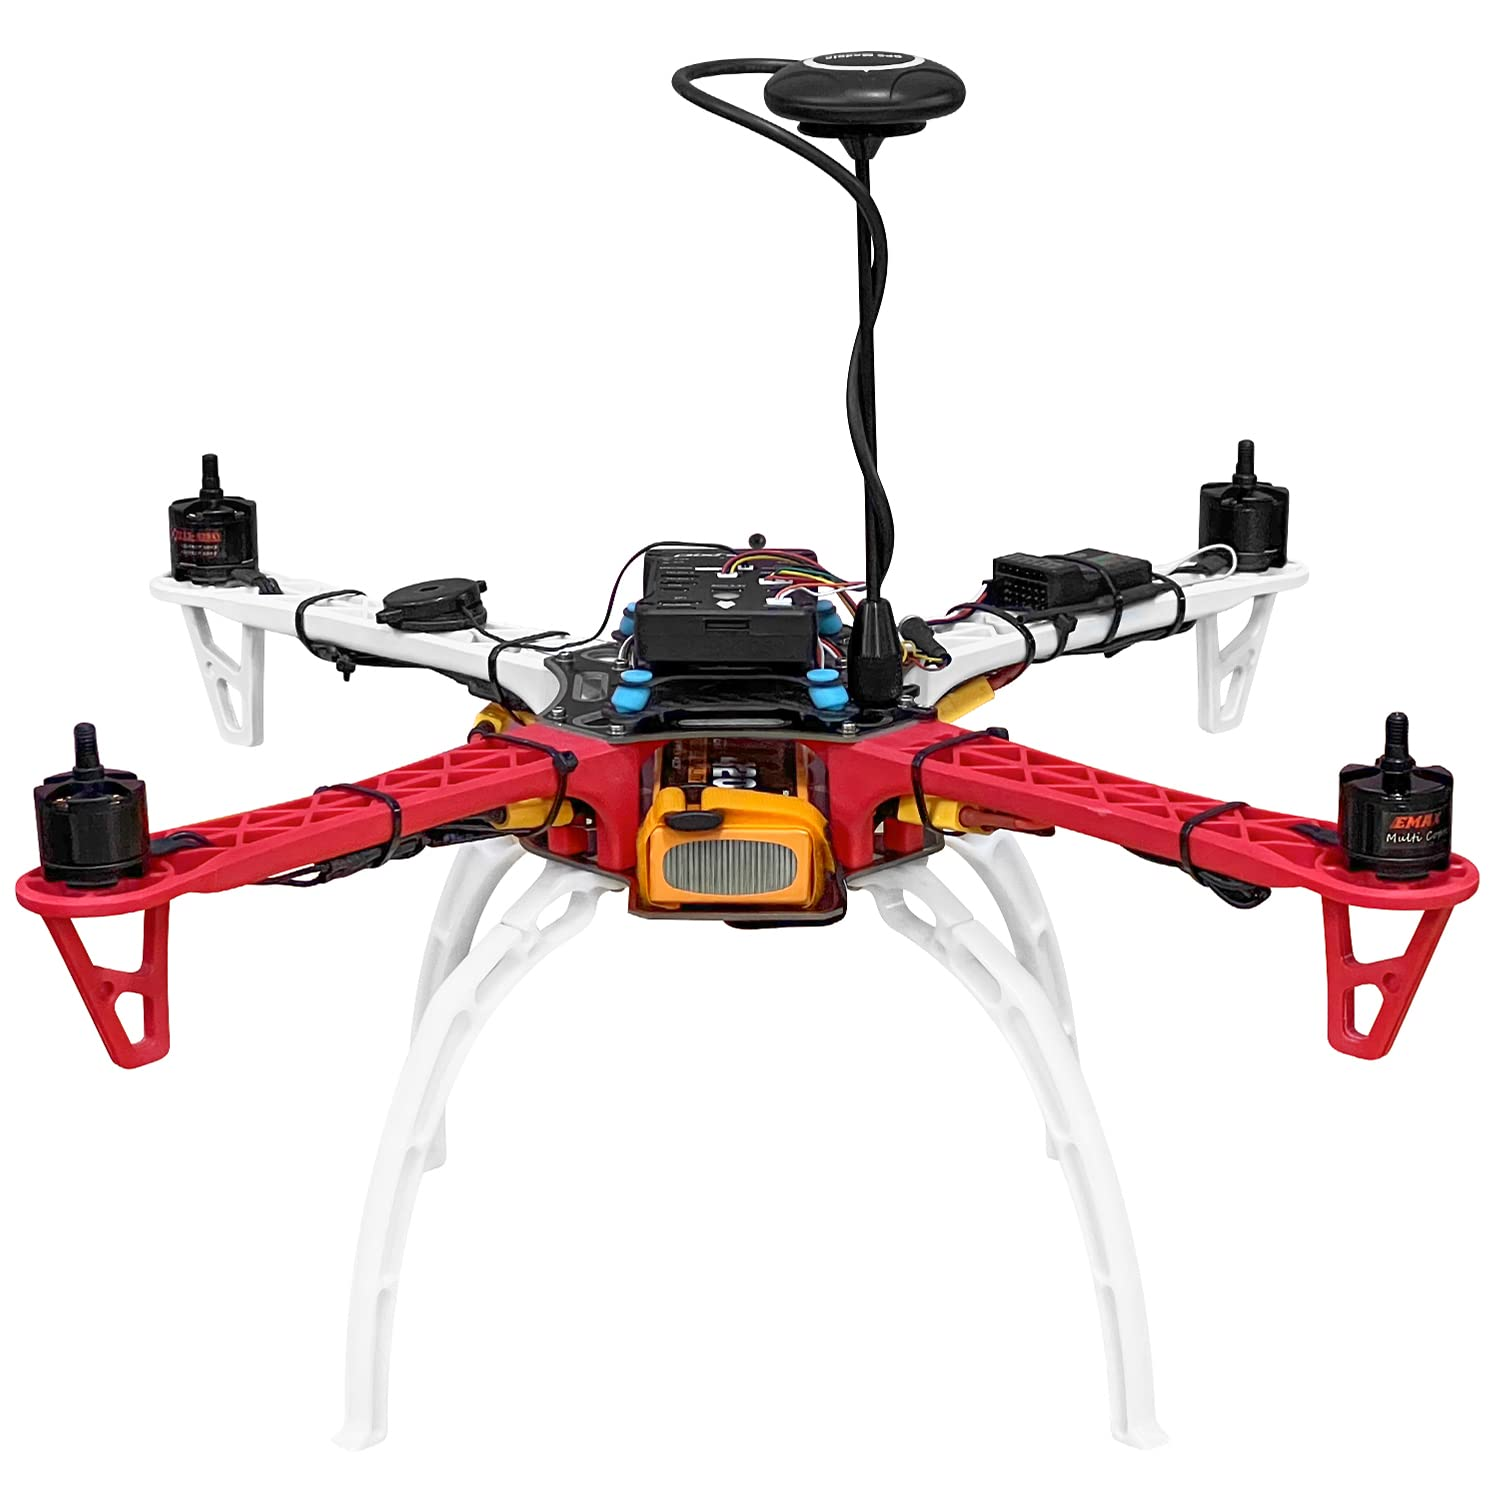
\includegraphics[scale=0.07]{img/f450.jpg} 
    \caption{Image of the generic F450 model. Source: Drones Company.}
    \label{fig:my_label}
\end{figure}

Building on this concept, a new drone was modeled with a modular design, allowing for easy disassembly of components. The new design protects wiring and equipment and includes a dedicated space for battery placement. The 3D modeling of the listed drone models was developed using the Tinkercad platform due to its intuitive interface, ease of use, and accessibility via a web browser, eliminating the need for a high-performance machine or any purchase or subscription.

Once the parts were designed, the project file was exported in ".STL" format to be sliced into layers using the FlashPrint software. This software generates a ".GX" file, which the printer recognizes to extrude material layer by layer, completing the manufacturing of the designed object.

The new parts were printed using PETG polymer on Flash Forge’s Guider IIs printer and GTMax3D’s A2v2 Core printer. PETG filament was selected for its combination of durability, toughness, flexibility, lightweight properties, and impact resistance, making it ideal for manufacturing robust drone components.

\subsection{IF450 Model}

\begin{figure}[!htb]
    \centering
    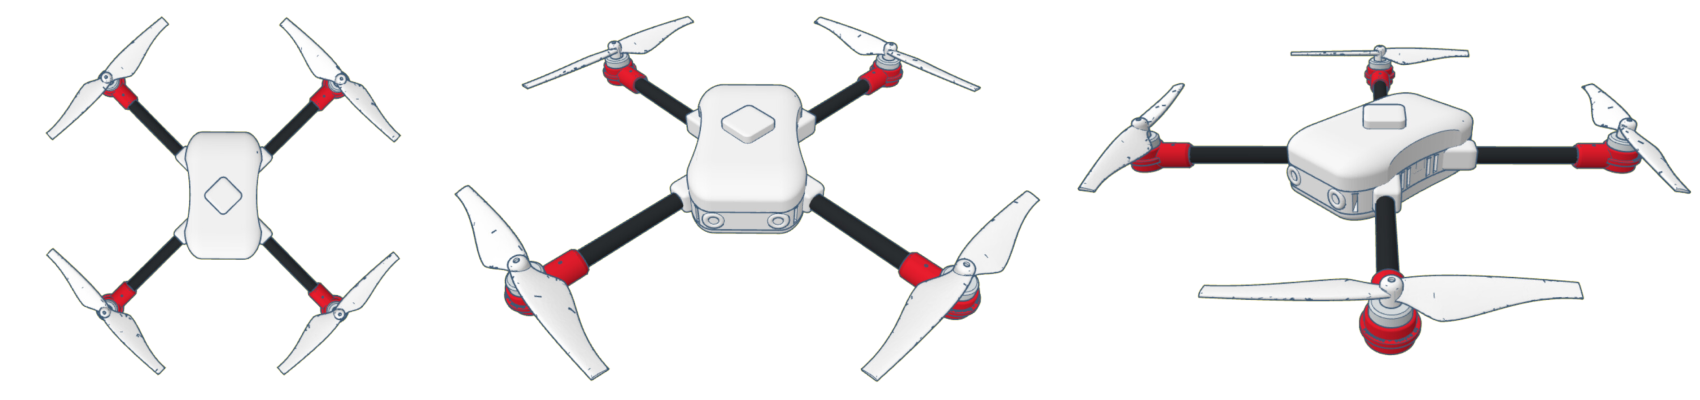
\includegraphics[scale=0.14]{img/IF450.png} 
    \caption{Three-dimensional model of the IF450 drone in Tinkercad. Source: Author}
    \label{fig:my_label}
\end{figure}

The IF450 model was designed with a closed structure and rounded edges, enhancing device protection and improving aerodynamics. Its arms are constructed from carbon fiber tubes with a 16 mm diameter and a 1 mm wall thickness. The design includes air inlets and outlets to facilitate cooling of the electronic system and features appropriate fittings for all mandatory equipment and peripheral accessories.

The new drone was named IF450, with "IF" representing the abbreviation for Instituto Federal (Federal Institute) and "450" indicating its size (the distance between motor axes). The central frame is composed of a single piece into which the carbon fiber arms fit, and the battery is mounted. The design incorporates two covers—one upper and one lower—secured by quick-release connectors and optionally four 2.5 mm diameter screws.

Removing these covers provides quick and easy access to the internal electronics, facilitating maintenance when needed. In addition to ensuring aerodynamics and protection, the design offers a clean and elegant aesthetic.

\subsection{Colibri Standard Model}

The drone is named after a hummingbird, Colibri, in homage to the city of Guanambi (meaning hummingbird in Tupi), with the suffix "Standard" to signify its role as the reference model for subsequent versions. Its design draws inspiration from the generic F450 model but incorporates minor modifications that result in significant positive impacts.

\begin{figure}[!htb]
    \centering
    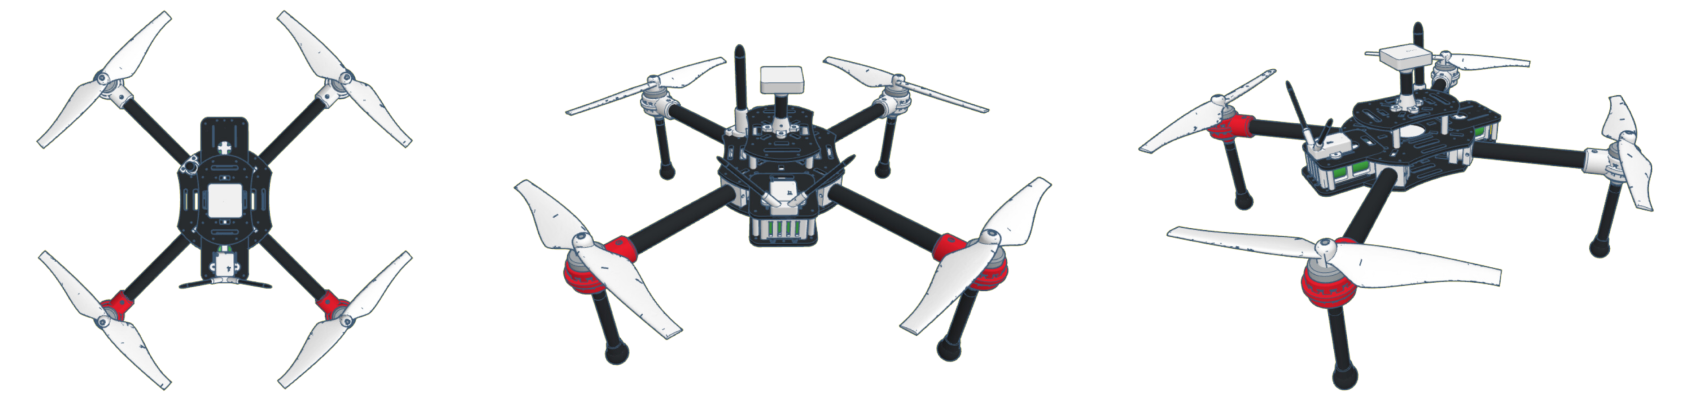
\includegraphics[scale=0.14]{img/Colibri-standard.png} 
    \caption{Three-dimensional model of the Colibri Standard drone in Tinkercad. Source: Author}
    \label{fig:my_label}
\end{figure}

The Colibri Standard maintains a 450 mm motor axis distance and features a central structure with a similar layout to the generic F450. However, it includes designated protected compartments for the flight controller and battery, which will be further detailed in the electronics section. The design employs carbon fiber tubular arms identical to those used in the IF450 (16 mm diameter and 1 mm wall thickness), enhancing durability, providing modularity, and safeguarding wires and devices housed within the arms. The landing gear is also constructed from carbon fiber tubes, though with a smaller diameter of 12 mm and the same 1 mm wall thickness.

Additionally, the frame includes a dedicated area for the power module and energy distribution system, as well as predefined holes to facilitate the integration of various accessories, including sensors and robotic mechanisms. The lower central area is kept free to accommodate additional equipment.

\subsection{Colibri Lite Model}

The Colibri Lite ("Lite" meaning "light" in Portuguese) also maintains a 450 mm motor axis distance. It offers similar functionalities to the Colibri Standard but is equipped with a smaller battery, fewer sensor connection points, and is designed for smaller flight controllers, making it a lighter version.

Its development was specifically aimed at competitions where weight plays a significant role in scoring, with autonomy becoming a secondary priority.

\begin{figure}[!htb]
    \centering
    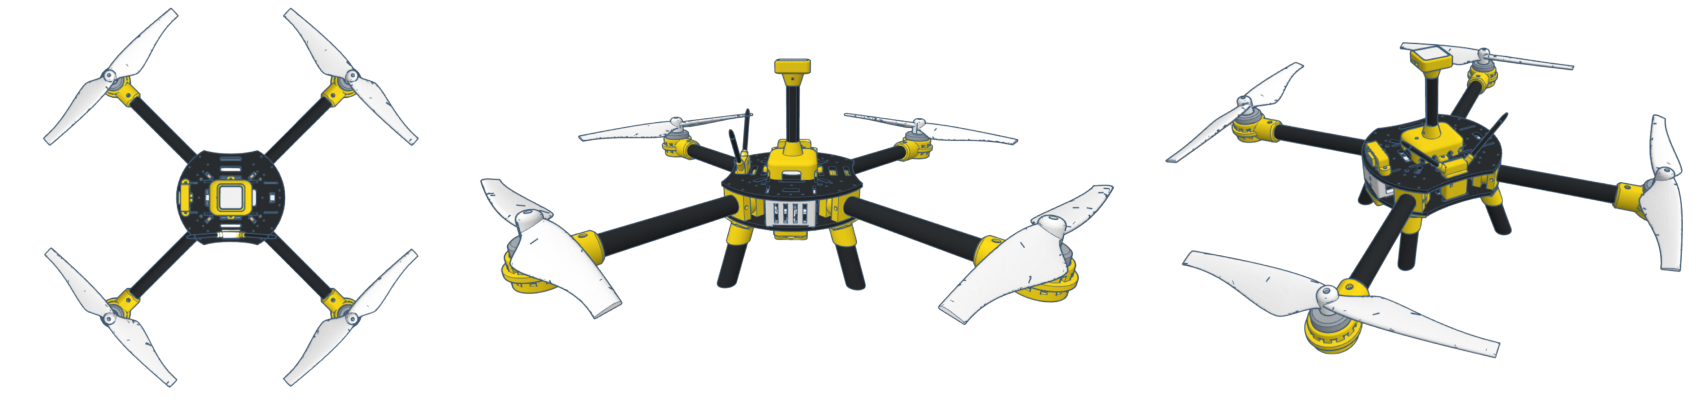
\includegraphics[scale=0.14]{img/Colibri-lite.png} 
    \caption{Three-dimensional model of the Colibri Lite drone in Tinkercad. Source: Author}
    \label{fig:my_label}
\end{figure}

\subsection{Colibri Mini Model}
The Colibri Mini is a smaller model with a 330 mm motor axis distance, making it the most compact among the Colibri series mentioned. It features 12 mm diameter carbon fiber tubular arms with a wall thickness of 1 mm. Essentially, it is a scaled-down version of the Colibri Standard.

Its development was initiated with competitions in mind, specifically those that restrict drones to sizes smaller than 450 mm. Although the default size is 330 mm, this dimension can be adjusted as needed.

\begin{figure}[!htb]
    \centering
    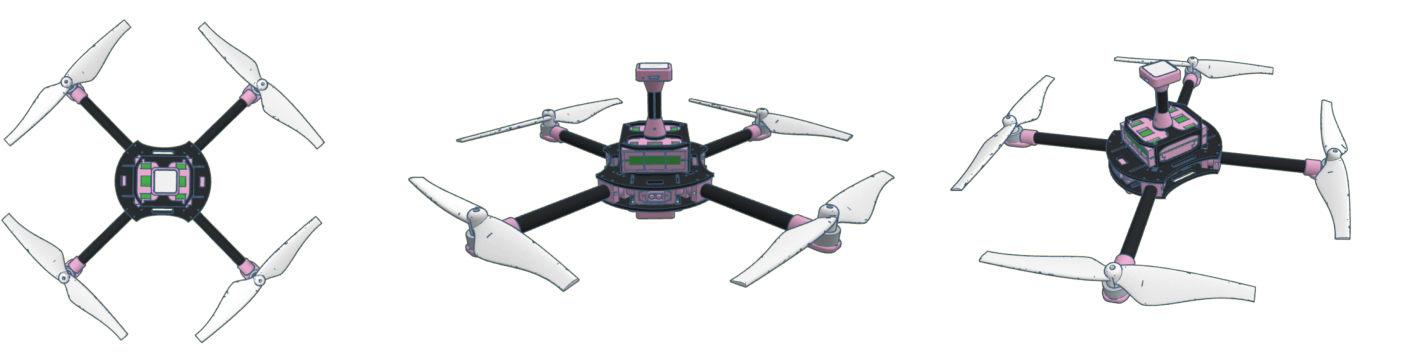
\includegraphics[scale=0.14]{img/Colibri-mini.png} 
    \caption{Three-dimensional model of the Colibri Mini drone in Tinkercad. Source: Author}
    \label{fig:my_label}
\end{figure}

\subsection{Colibri Micro Model}

The Colibri Micro is the most compact and lightweight model in the Colibri series, featuring a motor axis distance of 188 mm. It is the only model in the series with a structure entirely manufactured through additive manufacturing.

This model was designed for aerial missions in indoor environments or areas with numerous obstacles. Its robust, natively integrated propeller guards provide reduced vulnerability to damage and enhanced safety for animals and people.

\begin{figure}[!htb]
    \centering
    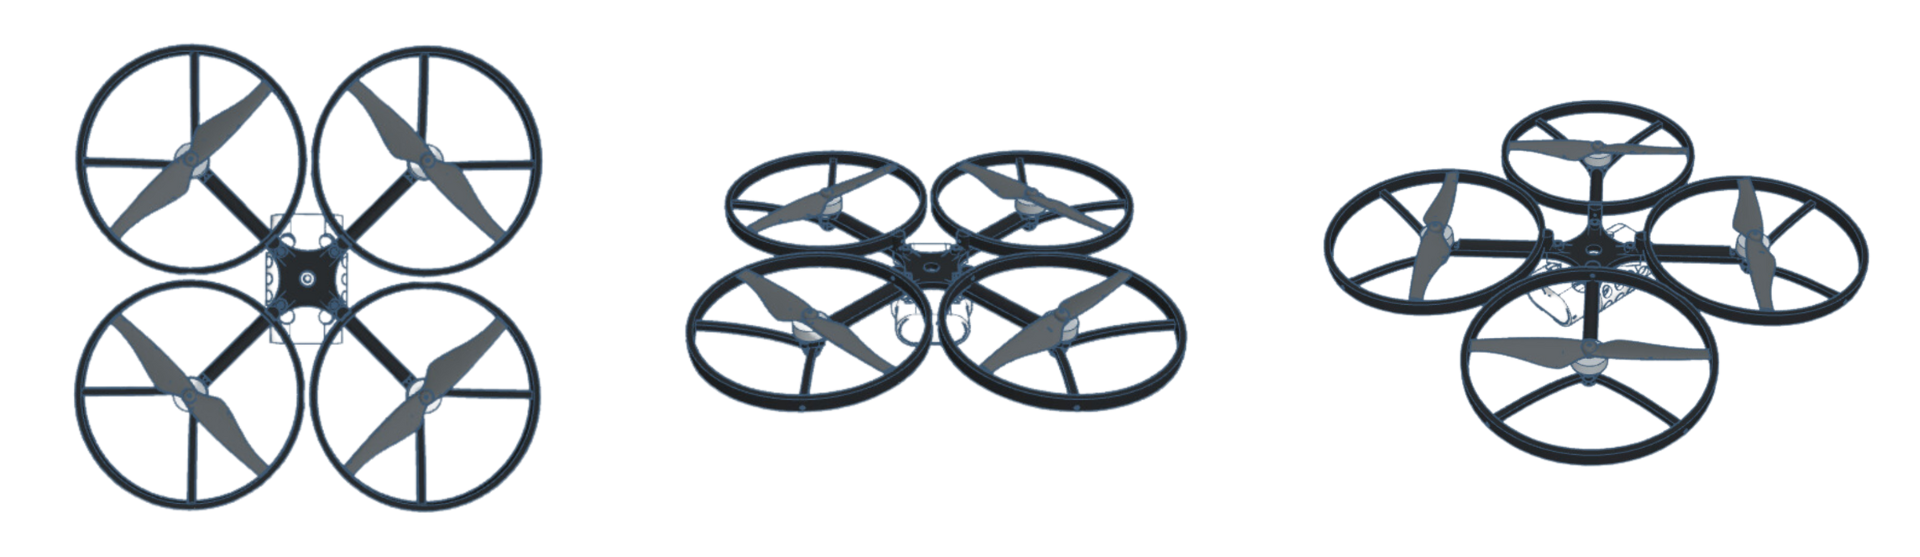
\includegraphics[scale=0.12]{img/Colibri-micro.png} 
    \caption{Three-dimensional model of the Colibri Micro drone in Tinkercad. Source: Author}
    \label{fig:my_label}
\end{figure}

\subsection{Colibri Hexa Model}
The Colibri Hexa, a six-rotor version, was developed to meet the requirements of the Drones IFSC competition for the H550 category. This category introduces a higher level of complexity in frame design due to the larger dimensions and the requirement for a 550 mm distance between opposing rotors and 60° spacing between each subsequent arm. Like the other versions, this model features 16 mm diameter carbon fiber tubular arms.

\begin{figure}[!htb]
    \centering
    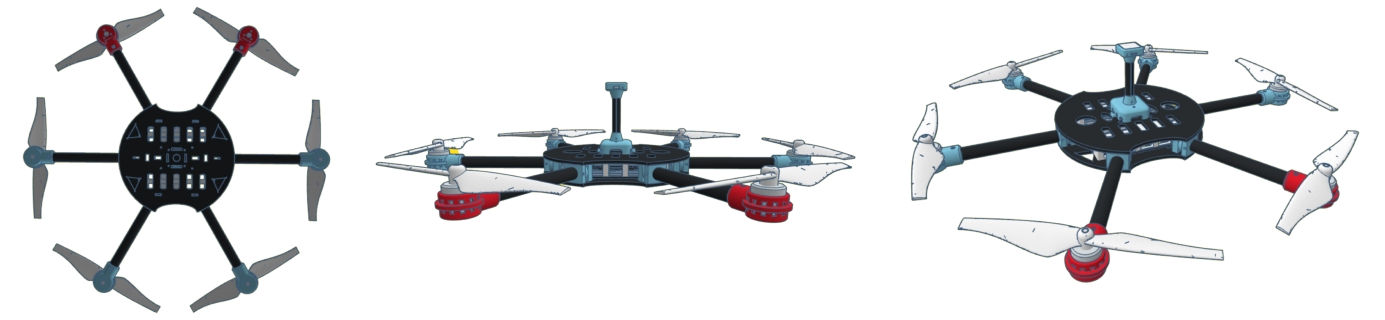
\includegraphics[scale=0.14]{img/Colibri-hexa.png} 
    \caption{Three-dimensional model of the Colibri Hexa drone in Tinkercad. Source: Author}
    \label{fig:my_label}
\end{figure}

The presence of six motors provides the drone with increased stability and redundancy, allowing the aircraft to remain in flight even if one motor fails. However, the larger frame dimensions and additional motors increase the drone's weight and power consumption. As a result, weight and energy efficiency become critical and limiting factors in fulfilling its intended uses.

\subsection{Electronic Components}

This section covers the propulsion system, flight controllers, integrated sensors, and other essential components that contribute to the functionality and performance of these unmanned aerial vehicles. Understanding these characteristics will clarify how design and technology choices directly influence their operational capabilities and efficiency.

All the developed drone versions share similar electronic components in the following aspects: Electronic Speed Controllers (ESC) utilizing BLHeli or SimonK firmware and connected to an 8-bit or 32-bit flight controller configured with Ardupilot firmware.

\begin{itemize}
    \item IF450 Model: The IF450 uses ESCs capable of handling 20 amperes, 800 KV brushless motors, 9” propellers, and a 6000 mAh lithium-ion battery pack manufactured by the team. Its flight controller is equipped with an 8-bit ATmega2560 microcontroller.
    
    \item Colibri Standard Model: The Colibri Standard is equipped with the same ESCs, motors, and propellers as the IF450, along with a 6000 mAh lithium-ion battery pack developed by the team. Its flight controller features a 32-bit STM32F427 microcontroller.
    
    \item Colibri Lite Model: The Colibri Lite utilizes the same ESC, motor, and propeller set as the Standard version but is designed to accommodate a smaller lithium-polymer battery with a 2500 mAh capacity and a flight controller based on the STM32F405RGT microcontroller. This configuration results in a lighter aircraft, offering a competitive advantage in events where weight is a decisive factor.

    \item Colibri Mini Model: The Colibri Mini features a frame design similar to the Lite version but at a reduced size. It is equipped with four 1400 KV motors, foldable 8” propellers, and a 20A 4-in-1 ESC configured with BLHeli firmware. This model supports a 3000 mAh lithium-polymer battery pack and a flight controller based on the STM32F405RGT microcontroller. The compact size allows this drone to compete in events requiring drones with motor axis distances of up to 330 mm.

    \item Colibri Micro Model: The Colibri Micro is equipped with a flight controller based on the 32-bit STM32H743VIT6 microcontroller, a 30A 4-in-1 ESC, 2824 KV motors with 6” propellers, and a 3000 mAh lithium-ion battery pack.

    \item Colibri Hexa Model: The Colibri Hexa employs the same ESC, motor, and propeller configuration as the Standard version, with modifications to the frame to accommodate two 3000 mAh lithium-polymer battery packs and a flight controller based on the STM32F405RGT microcontroller. The six-motor setup provides greater thrust, enabling the drone to carry heavier payloads compared to the other models.
    
\end{itemize}

For telemetry, all versions use the ESP32 module running Drone Bridge firmware. In combination with a 2.4 GHz WiFi router, this setup enables encrypted bidirectional MAVLink communication between the drone and the control station (computer or smartphone).

The GNSS positioning system in all versions uses a Ublox-M10050 receiver chip and a QMC5883L magnetometer. This system operates at a higher-than-normal frequency, supports all L1 GNSS signals (GPS, GLONASS, Galileo, BeiDou)—with up to three used simultaneously—and can navigate with up to 32 satellites at a 10 Hz update rate.

\section{Results and Discussion}

\begin{table}[htbp]
\centering
\caption{Comparison of Drone Models}
\label{tab:drone_comparison}
\begin{tabularx}{\columnwidth}{|l|X|X|X|}
\hline
\textbf{Model}         & \textbf{Operating Weight} & \textbf{Flight Time} & \textbf{Telemetry (Range)} \\ \hline
IF450                  & 1196 g                    & 24 min               & +300 m                     \\ \hline
Colibri Standard       & 1040 g                    & 28 min               & +300 m                     \\ \hline
Colibri Lite           & 788 g                     & 12 min               & +300 m                     \\ \hline
Colibri Mini           & 501 g                     & 28 min               & +300 m                     \\ \hline
Colibri Micro          & 275 g*                    & -                    & +300 m                     \\ \hline
Colibri Hexa           & -                         & -                    & +300 m                     \\ \hline
\end{tabularx}
\newline
\small *Estimated weight
\end{table}

The IF450 model has the highest weight among the tested 450 mm drones, weighing 1196 g. Conversely, the Colibri Lite is the lightest in the 450 mm class, with a weight of 788 g. Weight reduction is a critical factor, particularly in competitions where lighter drones can significantly enhance performance, as observed with the Colibri Lite. For competitions where drone size is not restricted, the Colibri Mini, Micro, and Hexa versions are excellent alternatives, with the Mini and Micro designed for indoor competitions with multiple obstacles, and the Hexa excelling in scenarios where payload capacity and flight stability are crucial for scoring.

Among the 450 mm class drones, the Colibri Standard demonstrated the longest flight time, with 28 minutes, followed by the IF450 at 24 minutes, and the Colibri Lite at 12 minutes. The 4-minute difference between the Colibri Standard and IF450 can be attributed to the lower weight of the Colibri Standard. In contrast, the Colibri Lite has a significantly shorter flight time of 12 minutes, due to its smaller lithium-polymer battery, which has a more limited voltage range compared to the lithium-ion batteries used in the other models.

The Colibri Mini also achieved a flight time of 28 minutes while being 34.3\% lighter than the Colibri Standard. All models demonstrate telemetry capabilities with a range exceeding 300 m, indicating robust communication suitable for most field applications. This range is sufficient for operations over areas up to 9 hectares.

\section*{Conclusions}

This study highlighted the distinctive characteristics of each drone model developed under the Educa Drones project, emphasizing their ideal applications based on weight, flight time, and telemetry capabilities. The ongoing development and evaluation of these drones could result in significant improvements in the efficiency and versatility of unmanned aerial vehicles.

For more comprehensive conclusions, additional data on the Colibri Micro and Colibri Hexa models is required. Future investigations should focus on collecting this data, as well as analyzing durability, maximum takeoff weight, and flight stability under adverse wind conditions. Moreover, comparisons with other commercial drones could provide a broader perspective on the competitiveness of the developed models.

\begin{thebibliography}{00}
\bibitem{b1} Abreu, J. V. V.; Bastos, B. L. (2015). Robótica Pedagógica e Currículo do Ensino Fundamental: Atuação em uma Escola Municipal do Projeto UCA. Revista Brasileira de Informática na Educação, v.23, n.3, 2015

\bibitem{b2} Brasil. Agência Nacional de Aviação Civil. (2023). Requisitos gerais para aeronaves não tripuladas de uso civil. RBAC-E94. Emenda n.3. Brasília, 2023.

\bibitem{b3} CBR, Competição Brasileira de Robótica. Disponível em: <https://cbr.robocup.org.br/index.php/categorias/> Acessado em de 30 junho 2024.

\bibitem{b4} IFSC, Competição de Drones IFSC Câmpus Florianópolis. Disponível em: <https://www.ifsc.edu.br/web/campus-florianopolis/veiculos-nao-tripulados-competicao-de-drones> Acessado em de 30 junho 2024.

\bibitem{b5} MNR, Mostra Nacional de Robótica. Disponível em: <https://mnr.robocup.org.br/> Acessado em de 30 junho 2024.

\bibitem{b6} OECD. PISA 2022 Results (Volume I): The State of Learning and Equity in Education. Paris: OCDE Publishing, 2023.

\bibitem{b7} SAE BRASIL. (2020). Fórmula Drone. Disponível em: <http://portal.saebrasil.org.br/programas-estudantis/sae-brasil-helidesign> Acesso: 20 de junho de 2020.

\bibitem{b8} Takagaki, L. K. (2012). Tecnologia de impressão 3D. Revista Inovação Tecnológica, São Paulo, v.2, n.2. p.2840. jul./dez.2012. 

\bibitem{b9} Ventura, A. A. O.; Albuquerque, J. L.; Praça Gomes, K. R. F.; Nascimento, S. M.; Leite, E. F.; Alves, J. L.; Diniz, J. R. B.; França, S. V. A. (2022). Robótica educacional e utilização de drones na educação: um mapeamento sistemático da literatura. Research, Society and Development, v. 11, n. 17, e251111739115, 2022.

\bibitem{b10} Wong, K. V.; Hernandez, A. A Review of Additive Manufacturing. ISRN Mechanical Engineering, v. 2012, p. 1–10, 2012

\bibitem{b11} Yepes, I. (2021). Uso de drones como Tecnologia pedagógica em disciplinas steam: um enfoque voltado ao aprendizado significativo com metodologias ativas. Tese (Doutorado) - Universidade Federal do Rio Grande do Sul, Centro de Estudos Interdisciplinares em Pós-Graduação em Informática na Educação. 2021, 240f. 

\bibitem{b12} Yepes, I.; Barone, D. A. C. (2018) Robótica Educativa: Proposta de uso de drones no apoio ao processo pedagógico em disciplinas STEM. Re, v(9). 2018. http://doi.org/10.5281/zenodo.1478926

\end{thebibliography}

\end{document}
